% Finished mode.
% \documentclass[nocolor]{article}
% \documentclass{article}

% Draft mode.
% \documentclass[working,nocolor]{article}
%\documentclass[working]{article}
\documentclass[working,a4paper]{article}
\usepackage[left=30mm,right=30mm,top=35mm,bottom=40mm]{geometry}

%%%%%%%%%%%%%%%%%%%%%%%%%%%%%%%%%%%%%%%%%%%%%%%%%%%%%%%%%%%%%%%%%%%%%%%%%%%%%%%
%                                Basic Packages                               %
%%%%%%%%%%%%%%%%%%%%%%%%%%%%%%%%%%%%%%%%%%%%%%%%%%%%%%%%%%%%%%%%%%%%%%%%%%%%%%%

% Gives us multiple colors.
\usepackage[usenames,dvipsnames,pdftex]{xcolor}
% Lets us style link colors.
\usepackage{hyperref}
% Lets us import images and graphics.
\usepackage{graphicx}
% Lets us use figures in floating environments.
\usepackage{float}
% Lets us create multiple columns.
\usepackage{multicol}
% Gives us better math syntax.
\usepackage{amsmath,amsfonts,amsthm,amssymb}
\usepackage{mathtools}
% Lets us strikethrough text.
\usepackage{cancel}
% Lets us edit the caption of a figure.
\usepackage{caption}
\usepackage{subcaption}
% Lets us import pdf directly in our tex code.
\usepackage{pdfpages}
% Lets us do algorithm stuff.
% \usepackage[ruled,vlined,linesnumbered]{algorithm2e}

\usepackage{algorithm}
\usepackage{algpseudocode}
\usepackage{bm}
% Use a smiley face for our qed symbol.
\usepackage{tikz}
\usepackage{tikzsymbols}
\usetikzlibrary{shapes,arrows,positioning}
% package for tables
\usepackage{booktabs}
\usepackage{multirow}
\usepackage{pifont}% http://ctan.org/pkg/pifont
\newcommand{\xmark}{\ding{55}}%
\usetikzlibrary{trees}
\usetikzlibrary{shapes,arrows,positioning}
\renewcommand\qedsymbol{$\Laughey$}
\DeclareMathOperator*{\argmax}{arg\,max}
\DeclareMathOperator*{\argmin}{arg\,min}
\def\class{article}



%%%%%%%%%%%%%%%%%%%%%%%%%%%%%%%%%%%%%%%%%%%%%%%%%%%%%%%%%%%%%%%%%%%%%%%%%%%%%%%
%                                Basic Settings                               %
%%%%%%%%%%%%%%%%%%%%%%%%%%%%%%%%%%%%%%%%%%%%%%%%%%%%%%%%%%%%%%%%%%%%%%%%%%%%%%%

%%%%%%%%%%%%%
%  Symbols  %
%%%%%%%%%%%%%

\let\implies\Rightarrow
\let\impliedby\Leftarrow
\let\iff\Leftrightarrow
\let\epsilon\varepsilon

%%%%%%%%%%%%
%  Tables  %
%%%%%%%%%%%%

\setlength{\tabcolsep}{5pt}
\renewcommand\arraystretch{1.5}

%%%%%%%%%%%%%%
%  SI Unitx  %
%%%%%%%%%%%%%%

\usepackage{siunitx}
\sisetup{locale = FR}

%%%%%%%%%%
%  TikZ  %
%%%%%%%%%%

\usepackage[framemethod=TikZ]{mdframed}
\usepackage{tikz}
\usepackage{tikz-cd}
\usepackage{tikzsymbols}

\usetikzlibrary{intersections, angles, quotes, calc, positioning}
\usetikzlibrary{arrows.meta}

\tikzset{
  force/.style={thick, {Circle[length=2pt]}-stealth, shorten <=-1pt}
}

%%%%%%%%%%%%%%%
%  PGF Plots  %
%%%%%%%%%%%%%%%

\usepackage{pgfplots}
\pgfplotsset{compat=1.13}

%%%%%%%%%%%%%%%%%%%%%%%
%  Center Title Page  %
%%%%%%%%%%%%%%%%%%%%%%%

\usepackage{titling}
\renewcommand\maketitlehooka{\null\mbox{}\vfill}
\renewcommand\maketitlehookd{\vfill\null}

%%%%%%%%%%%%%%%%%%%%%%%%%%%%%%%%%%%%%%%%%%%%%%%%%%%%%%%
%  Create a grey background in the middle of the PDF  %
%%%%%%%%%%%%%%%%%%%%%%%%%%%%%%%%%%%%%%%%%%%%%%%%%%%%%%%

\usepackage{eso-pic}
\newcommand\definegraybackground{
  \definecolor{reallylightgray}{HTML}{FAFAFA}
  \AddToShipoutPicture{
    \ifthenelse{\isodd{\thepage}}{
      \AtPageLowerLeft{
        \put(\LenToUnit{\dimexpr\paperwidth-222pt},0){
          \color{reallylightgray}\rule{222pt}{297mm}
        }
      }
    }
    {
      \AtPageLowerLeft{
        \color{reallylightgray}\rule{222pt}{297mm}
      }
    }
  }
}

%%%%%%%%%%%%%%%%%%%%%%%%
%  Modify Links Color  %
%%%%%%%%%%%%%%%%%%%%%%%%

\hypersetup{
  % Enable highlighting links.
  colorlinks,
  % Change the color of links to blue.
  linkcolor=blue,
  % Change the color of citations to black.
  citecolor={black},
  % Change the color of url's to blue with some black.
  urlcolor={blue!80!black}
}

%%%%%%%%%%%%%%%%%%
% Fix WrapFigure %
%%%%%%%%%%%%%%%%%%

\newcommand{\wrapfill}{\par\ifnum\value{WF@wrappedlines}>0
    \parskip=0pt
    \addtocounter{WF@wrappedlines}{-1}%
    \null\vspace{\arabic{WF@wrappedlines}\baselineskip}%
    \WFclear
\fi}

%%%%%%%%%%%%%%%%%
% Multi Columns %
%%%%%%%%%%%%%%%%%

\let\multicolmulticols\multicols
\let\endmulticolmulticols\endmulticols

\RenewDocumentEnvironment{multicols}{mO{}}
{%
  \ifnum#1=1
    #2%
  \else % More than 1 column
    \multicolmulticols{#1}[#2]
  \fi
}
{%
  \ifnum#1=1
\else % More than 1 column
  \endmulticolmulticols
\fi
}

\newlength{\thickarrayrulewidth}
\setlength{\thickarrayrulewidth}{5\arrayrulewidth}


%%%%%%%%%%%%%%%%%%%%%%%%%%%%%%%%%%%%%%%%%%%%%%%%%%%%%%%%%%%%%%%%%%%%%%%%%%%%%%%
%                           School Specific Commands                          %
%%%%%%%%%%%%%%%%%%%%%%%%%%%%%%%%%%%%%%%%%%%%%%%%%%%%%%%%%%%%%%%%%%%%%%%%%%%%%%%

%%%%%%%%%%%%%%%%%%%%%%%%%%%
%  Initiate New Counters  %
%%%%%%%%%%%%%%%%%%%%%%%%%%%

\newcounter{lecturecounter}

%%%%%%%%%%%%%%%%%%%%%%%%%%
%  Helpful New Commands  %
%%%%%%%%%%%%%%%%%%%%%%%%%%

\makeatletter

\newcommand\resetcounters{
  % Reset the counters for subsection, subsubsection and the definition
  % all the custom environments.
  \setcounter{subsection}{0}
  \setcounter{subsubsection}{0}
  \setcounter{paragraph}{0}
  \setcounter{subparagraph}{0}
  \setcounter{theorem}{0}
  \setcounter{claim}{0}
  \setcounter{corollary}{0}
  \setcounter{lemma}{0}
  \setcounter{exercise}{0}

  \@ifclasswith\class{nocolor}{
    \setcounter{definition}{0}
  }{}
}

%%%%%%%%%%%%%%%%%%%%%
%  Lecture Command  %
%%%%%%%%%%%%%%%%%%%%%

\usepackage{xifthen}

% EXAMPLE:
% 1. \lesson{Oct 17 2022 Mon (08:46:48)}{Lecture Title}
% 2. \lesson[4]{Oct 17 2022 Mon (08:46:48)}{Lecture Title}
% 3. \lesson{Oct 17 2022 Mon (08:46:48)}{}
% 4. \lesson[4]{Oct 17 2022 Mon (08:46:48)}{}
% Parameters:
% 1. (Optional) Lesson number.
% 2. Time and date of lecture.
% 3. Lecture Title.
\def\@lesson{}
\newcommand\lesson[3][\arabic{lecturecounter}]{
  % Add 1 to the lecture counter.
  \addtocounter{lecturecounter}{1}

  % Set the section number to the lecture counter.
  \setcounter{section}{#1}
  \renewcommand\thesubsection{#1.\arabic{subsection}}

  % Reset the counters.
  \resetcounters

  % Check if user passed the lecture title or not.
  \ifthenelse{\isempty{#3}}{
    \def\@lesson{Lecture \arabic{lecturecounter}}
  }{
    \def\@lesson{Lecture \arabic{lecturecounter}: #3}
  }

  % Display the information like the following:
  %                                                  Oct 17 2022 Mon (08:49:10)
  % ---------------------------------------------------------------------------
  % Lecture 1: Lecture Title
  \hfill\small{#2}
  \hrule
  \vspace*{-0.3cm}
  \section*{\@lesson}
  \addcontentsline{toc}{section}{\@lesson}
}


%%%%%%%%%%%%%%%%%%%%
%  Import Figures  %
%%%%%%%%%%%%%%%%%%%%

\usepackage{import}
\pdfminorversion=7

% EXAMPLE:
% 1. \incfig{limit-graph}
% 2. \incfig[0.4]{limit-graph}
% Parameters:
% 1. The figure name. It should be located in figures/NAME.tex_pdf.
% 2. (Optional) The width of the figure. Example: 0.5, 0.35.
\newcommand\incfig[2][1]{%
  \def\svgwidth{#1\columnwidth}
  \import{./figures/}{#2.pdf_tex}
}

\begingroup\expandafter\expandafter\expandafter\endgroup
\expandafter\ifx\csname pdfsuppresswarningpagegroup\endcsname\relax
\else
  \pdfsuppresswarningpagegroup=1\relax
\fi

%%%%%%%%%%%%%%%%%
% Fancy Headers %
%%%%%%%%%%%%%%%%%

\usepackage{fancyhdr}

% Force a new page.
\newcommand\forcenewpage{\clearpage\mbox{~}\clearpage\newpage}

% This command makes it easier to manage my headers and footers.
\newcommand\createintro{
  % Use roman page numbers (e.g. i, v, vi, x, ...)
  \pagenumbering{roman}

  % Display the page style.
  \maketitle
  % Make the title pagestyle empty, meaning no fancy headers and footers.
  \thispagestyle{empty}
  % Create a newpage.
  \newpage

  % Input the intro.tex page if it exists.
  \IfFileExists{intro.tex}{ % If the intro.tex file exists.
    % Input the intro.tex file.
    Lecture notes from the various YouTube playlist related to Reinforcement Learning, combined with the course E1277 Reinforcement Learning at
IISc Bangalore by Prof. Gugan Thoppe. The plan is to merge the notes from david silver's course and the course at IISc Bangalore,
at appropriate places, to make a single set of notes.

Since the notes are being merged from two different sources, proper crediting of the two (and many more) is hard. In general, the notes will follow, 
from the standard books of Reinforcement Learning, and are my interpretation of the same.

\textit{Disclaimer:} This document will inevitably contain some mistakes— both
simple typos and legitimate errors. Keep in mind that these are the notes of a graduate student in the process of learning the material, so take
what you read with a grain of salt. If you find mistakes and feel like telling
me, I will be grateful and happy to hear from you, even for the most trivial of
errors. You can reach me by email at
\href{mailto:vaidyavarad2001@gmail.com}{vaidyavarad2001@gmail.com}.

    % Make the pagestyle fancy for the intro.tex page.
    \pagestyle{fancy}

    % Remove the line for the header.
    \renewcommand\headrulewidth{0pt}

    % Remove all header stuff.
    \fancyhead{}

    % Add stuff for the footer in the center.
    \fancyfoot[C]{
      \textit{For more notes like this, visit
      \href{\linktootherpages}{\shortlinkname}}. \\
      \vspace{0.1cm}
      \hrule
      \vspace{0.1cm}
      \@author, \\
      \term: \academicyear, \\
      Last Update: \@date, \\
      \faculty
    }
  }{ % If the intro.tex file doesn't exist.
    % Force a \newpageage.
    \forcenewpage
  }

  % Create a new page.
  \newpage

  % Remove the center stuff we did above, and replace it with just the page
  % number, which is still in roman numerals.
  \fancyfoot[C]{\thepage}
  % Add the table of contents.
  \tableofcontents
  % Force a new page.
  \forcenewpage

  % Move the page numberings back to arabic, from roman numerals.
  \pagenumbering{arabic}
  % Set the page number to 1.
  \setcounter{page}{1}

  % Add the header line back.
  \renewcommand\headrulewidth{0.4pt}
  % In the top right, add the lecture title.
  \fancyhead[R]{\nouppercase{\leftmark}}
  % In the top left, add the author name.
  % In the bottom center, add the page.
  \fancyfoot[C]{\thepage}
  % Add a nice gray background in the middle of all the upcoming pages.
  % \definegraybackground
}

\makeatother


%%%%%%%%%%%%%%%%%%%%%%%%%%%%%%%%%%%%%%%%%%%%%%%%%%%%%%%%%%%%%%%%%%%%%%%%%%%%%%%
%                               Custom Commands                               %
%%%%%%%%%%%%%%%%%%%%%%%%%%%%%%%%%%%%%%%%%%%%%%%%%%%%%%%%%%%%%%%%%%%%%%%%%%%%%%%

%%%%%%%%%%%%
%  Circle  %
%%%%%%%%%%%%

\newcommand*\circled[1]{\tikz[baseline=(char.base)]{
  \node[shape=circle,draw,inner sep=1pt] (char) {#1};}
}

%%%%%%%%%%%%%%%%%%%
%  Todo Commands  %
%%%%%%%%%%%%%%%%%%%

\usepackage{xargs}
\usepackage[colorinlistoftodos]{todonotes}

\makeatletter

\@ifclasswith\class{working}{
  \newcommandx\unsure[2][1=]{\todo[linecolor=red,backgroundcolor=red!25,bordercolor=red,#1]{#2}}
  \newcommandx\change[2][1=]{\todo[linecolor=blue,backgroundcolor=blue!25,bordercolor=blue,#1]{#2}}
  \newcommandx\info[2][1=]{\todo[linecolor=OliveGreen,backgroundcolor=OliveGreen!25,bordercolor=OliveGreen,#1]{#2}}
  \newcommandx\improvement[2][1=]{\todo[linecolor=Plum,backgroundcolor=Plum!25,bordercolor=Plum,#1]{#2}}

  \newcommand\listnotes{
    \newpage
    \listoftodos[Notes]
  }
}{
  \newcommandx\unsure[2][1=]{}
  \newcommandx\change[2][1=]{}
  \newcommandx\info[2][1=]{}
  \newcommandx\improvement[2][1=]{}

  \newcommand\listnotes{}
}

\makeatother

%%%%%%%%%%%%%
%  Correct  %
%%%%%%%%%%%%%

% EXAMPLE:
% 1. \correct{INCORRECT}{CORRECT}
% Parameters:
% 1. The incorrect statement.
% 2. The correct statement.
\definecolor{correct}{HTML}{009900}
\newcommand\correct[2]{{\color{red}{#1 }}\ensuremath{\to}{\color{correct}{ #2}}}


%%%%%%%%%%%%%%%%%%%%%%%%%%%%%%%%%%%%%%%%%%%%%%%%%%%%%%%%%%%%%%%%%%%%%%%%%%%%%%%
%                                 Environments                                %
%%%%%%%%%%%%%%%%%%%%%%%%%%%%%%%%%%%%%%%%%%%%%%%%%%%%%%%%%%%%%%%%%%%%%%%%%%%%%%%

\usepackage{varwidth}
\usepackage{thmtools}
\usepackage[most,many,breakable]{tcolorbox}

\tcbuselibrary{theorems,skins,hooks}
\usetikzlibrary{arrows,calc,shadows.blur}

%%%%%%%%%%%%%%%%%%%
%  Define Colors  %
%%%%%%%%%%%%%%%%%%%

\definecolor{myblue}{RGB}{45, 111, 177}
\definecolor{mygreen}{RGB}{56, 140, 70}
\definecolor{myred}{RGB}{199, 68, 64}
\definecolor{mypurple}{RGB}{197, 92, 212}

\definecolor{definition}{HTML}{7B0000}
\definecolor{theorem}{HTML}{00007B}
\definecolor{example}{HTML}{000000}
\definecolor{definition}{HTML}{228b22}
\definecolor{prop}{HTML}{191971}
\definecolor{lemma}{HTML}{983b0f}
\definecolor{exercise}{HTML}{88D6D1}

% \colorlet{definition}{mygreen!85!black}
\colorlet{claim}{mygreen!85!black}
\colorlet{corollary}{mypurple!85!black}
\colorlet{proof}{theorem}
\colorlet{lemmaproof}{lemma}

%%%%%%%%%%%%%%%%%%%%%%%%%%%%%%%%%%%%%%%%%%%%%%%%%%%%%%%%%
%  Create Environments Styles Based on Given Parameter  %
%%%%%%%%%%%%%%%%%%%%%%%%%%%%%%%%%%%%%%%%%%%%%%%%%%%%%%%%%

\mdfsetup{skipabove=1em,skipbelow=0em}

%%%%%%%%%%%%%%%%%%%%%%
%  Helpful Commands  %
%%%%%%%%%%%%%%%%%%%%%%

% EXAMPLE:
% 1. \createnewtheoremstyle{thmdefinitionbox}{}{}
% 2. \createnewtheoremstyle{thmtheorembox}{}{}
% 3. \createnewtheoremstyle{thmproofbox}{qed=\qedsymbol}{
%       rightline=false, topline=false, bottomline=false
%    }
% Parameters:
% 1. Theorem name.
% 2. Any extra parameters to pass directly to declaretheoremstyle.
% 3. Any extra parameters to pass directly to mdframed.
\newcommand\createnewtheoremstyle[3]{
  \declaretheoremstyle[
  headfont=\bfseries\sffamily, bodyfont=\normalfont, #2,
  mdframed={
    #3,
  },
  ]{#1}
}

% EXAMPLE:
% 1. \createnewcoloredtheoremstyle{thmdefinitionbox}{definition}{}{}
% 2. \createnewcoloredtheoremstyle{thmexamplebox}{example}{}{
%       rightline=true, leftline=true, topline=true, bottomline=true
%     }
% 3. \createnewcoloredtheoremstyle{thmproofbox}{proof}{qed=\qedsymbol}{backgroundcolor=white}
% Parameters:
% 1. Theorem name.
% 2. Color of theorem.
% 3. Any extra parameters to pass directly to declaretheoremstyle.
% 4. Any extra parameters to pass directly to mdframed.
\newcommand\createnewcoloredtheoremstyle[4]{
  \declaretheoremstyle[
  headfont=\bfseries\sffamily\color{#2}, bodyfont=\normalfont, #3,
  mdframed={
    linewidth=2pt,
    rightline=false, leftline=true, topline=false, bottomline=false,
    linecolor=#2, backgroundcolor=#2!5, #4,
  },
  ]{#1}
}

%%%%%%%%%%%%%%%%%%%%%%%%%%%%%%%%%%%
%  Create the Environment Styles  %
%%%%%%%%%%%%%%%%%%%%%%%%%%%%%%%%%%%

\makeatletter
\@ifclasswith\class{nocolor}{
  % Environments without color.

  \createnewtheoremstyle{thmdefinitionbox}{}{}
  \createnewtheoremstyle{thmtheorembox}{}{}
  \createnewtheoremstyle{thmexamplebox}{}{}
  \createnewtheoremstyle{thmclaimbox}{}{}
  \createnewtheoremstyle{thmcorollarybox}{}{}
  \createnewtheoremstyle{thmpropbox}{}{}
  \createnewtheoremstyle{thmlemmabox}{}{}
  \createnewtheoremstyle{thmexercisebox}{}{}
  \createnewtheoremstyle{thmdefinitionbox}{}{}
  \createnewtheoremstyle{thmquestionbox}{}{}
  \createnewtheoremstyle{thmsolutionbox}{}{}

  \createnewtheoremstyle{thmproofbox}{qed=\qedsymbol}{}
  \createnewtheoremstyle{thmlemmaproofbox}{qed=\qedsymbol}{}
  \createnewtheoremstyle{thmexplanationbox}{}{}
}{
  % Environments with color.

  \createnewcoloredtheoremstyle{thmdefinitionbox}{definition}{}{}
  \createnewcoloredtheoremstyle{thmtheorembox}{theorem}{}{}
  \createnewcoloredtheoremstyle{thmexamplebox}{example}{}{
    % rightline=true, leftline=true, topline=true, bottomline=true
    backgroundcolor=white
  }
  \createnewcoloredtheoremstyle{thmclaimbox}{claim}{}{}
  \createnewcoloredtheoremstyle{thmcorollarybox}{corollary}{}{}
  \createnewcoloredtheoremstyle{thmpropbox}{prop}{}{}
  \createnewcoloredtheoremstyle{thmlemmabox}{lemma}{}{}
  \createnewcoloredtheoremstyle{thmexercisebox}{exercise}{}{}

  \createnewcoloredtheoremstyle{thmproofbox}{proof}{qed=\qedsymbol}{backgroundcolor=white}
  \createnewcoloredtheoremstyle{thmlemmaproofbox}{lemmaproof}{qed=\qedsymbol}{backgroundcolor=white}
  \createnewcoloredtheoremstyle{thmexplanationbox}{example}{qed=\qedsymbol}{backgroundcolor=white}
}
\makeatother

%%%%%%%%%%%%%%%%%%%%%%%%%%%%%
%  Create the Environments  %
%%%%%%%%%%%%%%%%%%%%%%%%%%%%%

\declaretheorem[numberwithin=section, style=thmtheorembox,     name=Theorem]{theorem}
\declaretheorem[numbered=no,          style=thmexamplebox,     name=Example]{example}
\declaretheorem[numberwithin=section, style=thmclaimbox,       name=Claim]{claim}
\declaretheorem[numberwithin=section, style=thmcorollarybox,   name=Corollary]{corollary}
\declaretheorem[numberwithin=section, style=thmpropbox,        name=Proposition]{prop}
\declaretheorem[numberwithin=section, style=thmlemmabox,       name=Lemma]{lemma}
\declaretheorem[numberwithin=section, style=thmexercisebox,    name=Exercise]{exercise}
\declaretheorem[numbered=no,          style=thmproofbox,       name=Proof]{replacementproof}
\declaretheorem[numbered=no,          style=thmlemmaproofbox,       name=Proof]{replacementlemmaproof}
\declaretheorem[numbered=no,          style=thmexplanationbox, name=Proof]{expl}
\declaretheorem[numberwithin=section, style=thmdefinitionbox,  name=Definition]{definition}

\makeatletter
\@ifclasswith\class{nocolor}{
  % Environments without color.

  \newtheorem*{note}{Note}

  \declaretheorem[numberwithin=section, style=thmquestionbox,   name=Question]{question}
  \declaretheorem[numberwithin=section, style=thmsolutionbox,   name=Solution]{solution}
}{
  % Environments with color.


  \newtcolorbox{note}[1][]{%
    enhanced jigsaw,
    colback=gray!20!white,%
    colframe=gray!80!black,
    size=small,
    boxrule=1pt,
    title=\textbf{Note:-},
    halign title=flush center,
    coltitle=black,
    breakable,
    drop shadow=black!50!white,
    attach boxed title to top left={xshift=1cm,yshift=-\tcboxedtitleheight/2,yshifttext=-\tcboxedtitleheight/2},
    minipage boxed title=1.5cm,
    boxed title style={%
      colback=white,
      size=fbox,
      boxrule=1pt,
      boxsep=2pt,
      underlay={%
        \coordinate (dotA) at ($(interior.west) + (-0.5pt,0)$);
        \coordinate (dotB) at ($(interior.east) + (0.5pt,0)$);
        \begin{scope}
          \clip (interior.north west) rectangle ([xshift=3ex]interior.east);
          \filldraw [white, blur shadow={shadow opacity=60, shadow yshift=-.75ex}, rounded corners=2pt] (interior.north west) rectangle (interior.south east);
        \end{scope}
        \begin{scope}[gray!80!black]
          \fill (dotA) circle (2pt);
          \fill (dotB) circle (2pt);
        \end{scope}
      },
    },
    #1,
  }

  \newtcbtheorem{Question}{Question}{enhanced,
    breakable,
    colback=white,
    colframe=myblue!80!black,
    attach boxed title to top left={yshift*=-\tcboxedtitleheight},
    fonttitle=\bfseries,
    title=\textbf{Question:-},
    boxed title size=title,
    boxed title style={%
      sharp corners,
      rounded corners=northwest,
      colback=tcbcolframe,
      boxrule=0pt,
    },
    underlay boxed title={%
      \path[fill=tcbcolframe] (title.south west)--(title.south east)
      to[out=0, in=180] ([xshift=5mm]title.east)--
      (title.center-|frame.east)
      [rounded corners=\kvtcb@arc] |-
      (frame.north) -| cycle;
    },
    #1
  }{def}

  \NewDocumentEnvironment{question}{O{}O{}}
  {\begin{Question}{#1}{#2}}{\end{Question}}

  \newtcolorbox{Solution}{enhanced,
    breakable,
    colback=white,
    colframe=mygreen!80!black,
    attach boxed title to top left={yshift*=-\tcboxedtitleheight},
    title=\textbf{Solution:-},
    boxed title size=title,
    boxed title style={%
      sharp corners,
      rounded corners=northwest,
      colback=tcbcolframe,
      boxrule=0pt,
    },
    underlay boxed title={%
      \path[fill=tcbcolframe] (title.south west)--(title.south east)
      to[out=0, in=180] ([xshift=5mm]title.east)--
      (title.center-|frame.east)
      [rounded corners=\kvtcb@arc] |-
      (frame.north) -| cycle;
    },
  }

  \NewDocumentEnvironment{solution}{O{}O{}}
  {\vspace{-10pt}\begin{Solution}{#1}{#2}}{\end{Solution}}
}
\makeatother

%%%%%%%%%%%%%%%%%%%%%%%%%%%%
%  Edit Proof Environment  %
%%%%%%%%%%%%%%%%%%%%%%%%%%%%

\renewenvironment{proof}[1][\proofname]{\vspace{-10pt}\begin{replacementproof}}{\end{replacementproof}}
\newenvironment{explanation}[1][\proofname]{\vspace{-10pt}\begin{expl}}{\end{expl}}
\newenvironment{lemmaproof}[1][\proofname]{\vspace{-10pt}\begin{replacementlemmaproof}}{\end{replacementlemmaproof}}
\theoremstyle{definition}

\newtheorem*{notation}{Notation}
\newtheorem*{previouslyseen}{As previously seen}
\newtheorem*{problem}{Problem}
\newtheorem*{observe}{Observe}
\newtheorem*{property}{Property}
\newtheorem*{intuition}{Intuition}

%%%%%%%%%%%%%%%%%%%%%%%%%
% Autoref Configuration %
%%%%%%%%%%%%%%%%%%%%%%%%%
\makeatletter
\newcommand\tcb@cnt@Definitionautorefname{Definition}
\makeatother
\newcommand{\algorithmautorefname}{Algorithm}

%%%%%%%%%%%%%%
% part on a seperate page
%%%%%%%%%%%%%%

\makeatletter
\renewcommand\part{%
%  \if@openright
%    \cleardoublepage
%  \else
    \clearpage
%  \fi
  \thispagestyle{plain}%
  \if@twocolumn
    \onecolumn
    \@tempswatrue
  \else
    \@tempswafalse
  \fi
  \null\vfil
  \secdef\@part\@spart}

\def\@part[#1]#2{%
    \ifnum \c@secnumdepth >-2\relax
      \refstepcounter{part}%
      \addcontentsline{toc}{part}{\thepart\hspace{1em}#1}%
    \else
      \addcontentsline{toc}{part}{#1}%
    \fi
    \markboth{}{}%
    {\centering
     \interlinepenalty \@M
     \normalfont
     \ifnum \c@secnumdepth >-2\relax
       \huge\bfseries \partname\nobreakspace\thepart
       \par
       \vskip 20\p@
     \fi
     \Huge \bfseries #2\par}%
    \@endpart}
    
\def\@spart#1{%
    {\centering
     \interlinepenalty \@M
     \normalfont
     \Huge \bfseries #1\par}%
    \@endpart}
\def\@endpart{\vfil\newpage}
\makeatother

\usepackage{lipsum} % For random text. You don't need this.
\title{Reinforcement Learning Notes}
\author{Varad Vaidya}
\date{\today}

\newcommand{\linktootherpages}{varadvaidya.github.io}
\newcommand{\shortlinkname}{varadVaidya}
\newcommand{\term}{Fall Term}
\newcommand{\academicyear}{$2023$}
\newcommand{\faculty}{}

\begin{document}
  \createintro

  % start lectures  
  \input{david_silver/lec1}
  \clearpage
  `\section{{Lecture 2 | Markov Decision Processes}}
Markov decision process formally describe an enviroment for reinforcement
learning. The nice case for this setting is that the environemtn is fully observable. Thus,
the current state completely characterizes the process. This is called the Markov property.

Thus, all RL problems can bve formalised in terms of MDPs. Optimal Control problem can be 
formalised as continuous MDPs. Partially observable problems can be always converted 
to MDPs.
\subsection{Markov Processes or Markov Chains}
A Markov chain is simply a Markov Decision Process without decision. It is one the 
most simplest stocastic process, and has no ``memory'' of the past. So, just the 
present stat determines its future dynamics. In this context, we will be considering
Discrete Time Markov Chains (DTMCs).

DTMC involves two concepts:
\begin{itemize}
    \item Discrete Time Stochastic Process (DTSP)
    \item Row Stochastic Matrix.
\end{itemize}

The two are defined as follows:

\begin{definition}[Discrete Time Stochastic Process (DTSP)]
    A DTSP is a sequence \({(X_n)}_{n \geq 0}\) of random variables defined on the same proboability space
    \((\Omega, \mathcal{F} , \mathbb{P} )\), taking values in the same 
    set \(\mathcal{S} \), i.e.
    \[
        X_n : \Omega \rightarrow \mathcal{S} \quad \forall n \geq 0
    \]
\end{definition}
where \(\mathcal{S} \) is called a state space, and in finite or countably infinite.
We call the a variable as a ``state'' when the state is an element of the state space \(\mathcal{S} \).
The cardinality of the state space is denoted by \(|\mathcal{S} |\).

\begin{definition}[Row Stochastic Matrix]
    A matrix \(\mathcal{P} \in \mathbb{R}^{|S| \times |S|}\) is called a row stochastic matrix if
    it satisfies the following conditions:
    \[
        \mathcal{P} _{ij} \in [0, 1] \quad \forall i, j \in \mathcal{S}  
    \]
    \[
        \sum\limits_{j = 1 }^{ |\mathcal{S}|} \mathcal{P} _{ij} = 1 \quad \forall i \in \mathcal{S}  
    \]
\end{definition}
Thus, with these two definitions we can define a Markov Chain (or DTMC) as follows:
\begin{definition}[Markov Chain]
    Let \(\mathcal{S} \) be a finite state space, and \(\nu\) be a distribution over \(\mathcal{S} \).
    \[
        \nu = (\nu _{1}, \nu _{2}, \dots, \nu _{|\mathcal{S}|}) \quad
        \text{s.t} \quad \nu _{i} \in [0, 1] \; \forall i \in \mathcal{S},
        \quad \sum\limits_{i \in \mathcal{S} } \nu _{i} = 1
    \]  
    Further, let \(\mathcal{P} \) be a row stocastic matrix over \(\mathcal{S} \).
    
    Then a DTSP \({(X_n)}_{n \geq 0}\) is called a Markov Chain with initial distribution \(\nu \)
    and transition matrix \(\mathcal{P} \) if it satisfies the following conditions:
    \begin{itemize}
        \item Initial state is distributed according to \(\nu \), i.e.
        \[
            \mathbb{P}(X_0 = i) = \nu _{i} \quad \forall i \in \mathcal{S}    
        \]
        \item Present is independent of the past given the present.
        \[
            \begin{aligned}
                \mathbb{P} \left( 
                    X_{n+1} = i_{n+1} | X_{n} = i_{n}, X_{n-1} = i_{n-1}, \dots, X_{0} = i_{0}
                 \right) &= \mathbb{P} \left( 
                     X_{n+1} = i_{n+1} | X_{n} = i_{n}
                  \right) \\
                    & = \mathcal{P}_{i_{n} i_{n+1}} \quad \forall n \geq 0
            \end{aligned}
        \]
    \end{itemize}
\end{definition}

\begin{example}[Markov Chains]
    Let a Markov chain be defined as follows:
    \[
        \mathcal{S}  = \{1,2\} \quad \nu = (p, 1-p) \quad \mathcal{P}  = \begin{bmatrix}
            1-\alpha  &  \alpha  \\
            \beta  &  1-\beta  \\
        \end{bmatrix}
    \]
    \begin{center}
        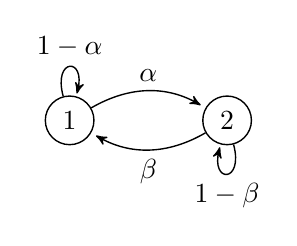
\begin{tikzpicture}[->,>=stealth',shorten >=2pt,line width=0.5pt,node distance=2cm]
            \node[circle,draw] (zero) {1};
            \node[circle,draw] (one) [right of=zero] {2};
            \path (zero) edge [loop above] node {\(1-\alpha \)} (zero);
            \path (zero) edge [bend left] node[above] {\(\alpha \)} (one);
            \path (one) edge [loop below] node {\(1-\beta \)} (one);
            \path (one) edge [bend left] node[below] {\(\beta \)} (zero);
        \end{tikzpicture}
    \end{center}
Thus, we can have say:
\[
    \mathbb{P} (X_3 = 1 | X_0 = 1, X_1 = 1 , X_2 - 2) = \beta 
\]

Another example that we can have is:
\[
    \mathcal{S} = \{1,2,3\} \quad \nu = (\nu_{1}, \nu_{2}, \nu_{3}) \quad \mathcal{P} = \begin{bmatrix}
        0 & 1 & 0 \\
        0 & \frac{1}{2} & \frac{1}{2}  \\
        \frac{1}{2} & 0 & \frac{1}{2} \\
    \end{bmatrix}
\]
    \begin{center}
        \begin{tikzpicture}[->,>=stealth',shorten >=2pt,line width=0.5pt,node distance=3cm]
            \node[circle,draw] (one) {1};
            \node[circle,draw] (two) [below right of=zero] {2};
            \node[circle,draw] (three) [below left of=zero] {3};
            \path (one) edge [bend left] node[below left] {\(1 \)} (two);
            \path (two) edge [bend left] node[above] {\(\frac{1}{2} \)} (three);
            \path (three) edge [bend left] node[below right] {\(\frac{1}{2} \)} (one);
        \end{tikzpicture}
    \end{center}
    given, \(\nu = (1,0,0)\), the outcomes of the Markov chain if we sample it are:
    \[
        \begin{aligned}
            X_n &= 1, 2, 3, 3, 1, 2, \dots \\
            &= 1, 2, 3, 1, 2, \dots \\ 
        \end{aligned}
    \] 
\end{example}
\vspace{1em}
Note that, to define the DTMC, we need the initial distribution, but the results wont change on the
choice of the distribution \(\nu\), assuming that the Markov chain is ergodic. Hence, while
defining the markov chain, the initial distribution is not mentioned, and can be assumed
arbitrarily.


% \subsubsection*{State Transition Matrix}
% For a markov state \(s\) and succesor state \(s^{\prime} \) the state transition probability
% is defined as:
% \begin{equation}
%     \mathcal{P} _{ss^{\prime}} = \mathcal{P} [S_{t+1} = s^{\prime} | S_{t} = s]
% \end{equation}
% Thus each row of the matrix is a probability distribution over the next state assuming
% that we are in the state of the row. 
% \[
%     \mathcal{P} = 
%     \begin{bmatrix}
%         \mathcal{P} _{11} & \mathcal{P} _{12} & \dots & \mathcal{P} _{1n} \\
%         \mathcal{P} _{21} & \mathcal{P} _{22} & \dots & \mathcal{P} _{2n} \\
%         \vdots & \vdots & \ddots & \vdots \\
%         \mathcal{P} _{n1} & \mathcal{P} _{n2} & \dots & \mathcal{P} _{nn} \\
%     \end{bmatrix}  
% \]
% Each row sums over to 1.

% THus, a markov process is a memoeryless random process, i.e. a sequence of random states
% \(S_{1}, S_{2}, \dots \) with the Markov property. 

% \begin{definition}[Markov Process]
%     A Markov process is a tuple \((\mathcal{S}, \mathcal{P} )\) consisting of a finite set
%     of states \(\mathcal{S} \) and a state transition probability matrix \(\mathcal{P} \).
%     where,
%     \[
%         \mathcal{P} _{ss^{\prime}} = \mathbb{P}  [S_{t+1} = s^{\prime} | S_{t} = s]  
%     \]
%     for all \(s, s^{\prime} \in \mathcal{S} \).
% \end{definition}
% Random Process is a random sequence that is drawn from a probability distribution over 
% the sequences of state given by the markov chain.

\begin{theorem}[Necessary and Sufficient Conditions for DTSP to be Markov Chains]
    A DTSP \({(X_n)}_{n \geq 0}\) on \(\mathcal{S}\)  is a Markov chain \(\langle \mathcal{S} , \mathcal{P} 
    ,\nu \rangle\) if and only if:
    \[
        \mathbb{P} \left( 
            X_{n} = i_{n} , X_{n} = i_{n}, \dots, X_{0} = i_{0}
            \right) = \nu _{i_{0}} \mathcal{P} _{i_{0} i_{1}}
             \mathcal{P} _{i_{1} i_{2}} \dots \mathcal{P} _{i_{n-1} i_{n}} \quad \forall n \geq 0
    \] 
\end{theorem}
\begin{proof}
    To simplify the proof, assume that \(\mathcal{P}_{ij} > 0 \quad \forall i, j \in \mathcal{S} \).
    The theorem remains true in the general case, but requires more book-keeping.

    Suppose, \({(X_n)}_{n \geq 0}\) is a Markov chain \(\langle \mathcal{S} , \mathcal{P}
    , \nu \rangle\). 
    
    Using the fact,
    \[
        \begin{aligned}
            \mathbb{P}(A \cap B) &= \mathbb{P}(A) \mathbb{P}(B | A) \\
            \mathbb{P}(A \cap B \cap C) &= \mathbb{P}(A) \mathbb{P}(B | A) \mathbb{P}(C | A \cap B) \\
        \end{aligned}
    \]
    We get,
    \[
        \begin{aligned}
            \mathbb{P}(X_0 = i_0, \dots , X_n = i_n)  & = \mathbb{P} \left( 
                \{X_0 = i_0\} \cap \{X_1 = i_1\} \cap \dots \cap \{X_n = i_n\}
             \right)\\ 
             & = \mathbb{P}(X_0 = i_0) \mathbb{P}(X_1 = i_1 | X_0 = i_0) \dots \mathbb{P}(X_n = i_n | X_{n-1} = i_{n-1}) \\
             & = \mathbb{P} (X_0 = i_0) \mathbb{P}(X_1 = i_1 | X_0 = i_0) \dots \mathbb{P}(X_n = i_n | X_{n-1} = i_{n-1}) \\
             &\dots  \text{Using the memoeryless property of Markov chains} \\
                & = \nu _{i_0} \mathcal{P} _{i_0 i_1} \dots \mathcal{P} _{i_{n-1} i_n} \\
        \end{aligned}
    \]

    This proves the forward claim. To show the reverse claim:

    Put \(n=0\), in the claim, to trivially get the initial distribution back, showing one part of the definition.
    For the other part:
    \[
    \begin{aligned}    
        \mathbb{P}(X_{n} = i_{n} | X_{n-1} = i_{n-1}, \dots, X_{0} = i_{0}) &=
         \frac{\mathbb{P}(X_{n} = i_{n}, \dots, X_{0} = i_{0})}
         {\mathbb{P}(X_{n-1} = i_{n-1}, \dots, X_{0} = i_{0})} \\
         &= \frac{\nu _{i_0} \mathcal{P} _{i_0 i_1} \dots \mathcal{P} _{i_{n-1} i_n}}
         {\nu _{i_0} \mathcal{P} _{i_0 i_1} \dots \mathcal{P} _{i_{n-1} i_n}} \\
            &= \mathcal{P} _{i_{n-1} i_n} \\
    \end{aligned}
    \]

    Now we need to show:
    \[
        \mathbb{P}(X_{n} = i_{n} | X_{n-1} = i_{n-1})
    \]
    \[
        \begin{aligned}
            & = \frac{\mathbb{P}(X_{n-1} = i_{n-1}, X_{n} = i_{n})}{\mathbb{P}(X_{n-1} = i_{n-1})} \\
            & = \frac{\sum_{i_0 \in \mathcal{S} } \mathbb{P}(X_0 = i_0 \dots  X_{n-1} = i_{n-1}, X_{n} = i_{n})}
            {\sum_{i_0 \in \mathcal{S} } \mathbb{P}(X_{n-1} = i_{n-1}, X_{0} = i_{0})} \\
            & = \mathcal{P} _{i_{n-1} i_n} \\
        \end{aligned}
    \]
\end{proof}\vspace{1em}
In the above proof we have used the following series of fact:
\[
    \begin{aligned}
        \mathbb{P} (X_2 = j) & = \mathbb{P}(\Omega \cap \{X_2 = j\})\\
        &= \mathbb{P} \left[ 
            \bigcup_{i=1}^{ |S| } \{X_i = i\} \cap \{X_2 = j\}
         \right] \\
    \end{aligned}
\]
Using the fact:
\[
    (A \cup B) \cap C = (A \cap C ) \cup (B \cap C)
\]
we get:
\[
    \begin{aligned}
        \mathbb{P} (X_2 = j) & = \sum\limits_{i = 1}^{ |S| } 
        \mathbb{P} \left(
             X_i = i, X_2 = j
         \right)
    \end{aligned}
\]

\begin{theorem}[Markov Property]
    Let \({(X_n)}_{n \geq  0} \) be the markov chain detnoted by \(\langle \mathcal{S} ,\mathcal{P} ,\mu  \rangle \),
then condintional on \(\{X_m = i\}\), \(\{X_{m+n} \}\) is the markov chain \(\langle \mathcal{S} ,\mathcal{P} , \delta _i \rangle \) 
and is independent of \(X_1, X_2, \dots , X_m\), where \(\delta _i\) is the distribution that is 1 at \(i\)
 and 0 everywhere else, i.e
 \[
        \delta _i (j) \equiv \delta_{ij} =  \begin{cases}
            1 & \text{if } j = i \\
            0 & \text{otherwise} \\
        \end{cases} 
 \]
\end{theorem}
\begin{proof}
    It suffices to show the following, for any \(n \geq 0\) and on an event \(A\), related to \(X_0,\dots , X_m\):
    \[
        \begin{aligned}
            \mathbb{P} \left[ 
                (X_m = i_m, X_{m+1} = i_{m+1}, \dots , X_{m+n} = i_{m+n}) \cap A \mid X_m = i_m 
                \right] \\ 
                = \mathbb{P} ( A \mid X_m=i_m) \delta_{ij} \mathcal{P} _{i_m i_{m+1}} \dots 
                \mathcal{P} _{i_{m+n-1} i_{m+n}} 
            \end{aligned}
    \]
    The above equation is just conditional independence:
    \[
        \mathbb{P} (E_1 \cap  E_2 \mid X_m = i) = \mathbb{P} (E_1 \mid X_m = i) \mathbb{P} (E_2 \mid X_m = i)
    \]
    where \(E_2 = (X_m = i_m, X_{m+1} = i_{m+1}, \dots , X_{m+n} = i_{m+n})\) and \(E_1 = A\). The proof of the above statement goes as follows:

    Let \(A\) be an elementary event, i.e. \(A = \{X_0 = j_0, X_1 = j_1, \dots , X_m = j_m\}\). Consider the LHS of the above equation:
    Then, we have two cases:
    \begin{itemize}
        \item \textbf{Case 1}: \(j_m \neq i_m\). Then, the LHS is trivially 0, since \(A\) and \(E_2\) are disjoint.
        \item \textbf{Case 2}: \(j_m = i_m\). Then, we have further cases. When, \( i \neq i_m = j_m\), then 
        the LHS and RHS are again 0. But when \(i = i_m = j_m\), then the LHS is: 
        \begin{multline*}
        \begin{aligned}
                \mathbb{P} (
                    X_0 = j_0, X_1 = j_1, \dots X_m = j_m = i ,X_m = i_m = i, X_{m+1} = i_{m+1},\\ \dots , X_{m+n} = i_{m+n} \mid X_m = i_m = i 
                    )
                \end{aligned}
            \end{multline*}
            \[
                \begin{aligned}
                    &= \frac{\nu(j_o) \mathcal{P}_{j_0 j_1} \dots \mathcal{P}_{j_{m-1} j_m} 
                    \mathcal{P}_{j_m i_{m+1}} \dots \mathcal{P}_{i_{m+n-1} i_{m+n}}}
                    {\mathbb{P} (X_m = i_m = i)} \\
                    &= \frac{\mathbb{P} (A) \mathcal{P}_{i_m i_{m+1}} \dots \mathcal{P}_{i_{m+n-1} i_{m+n}}}
                    {\mathbb{P} (X_m = i_m = i)} \\
                    &= \mathbb{P} (A \mid X_m = i_m = i) \mathcal{P}_{i_m i_{m+1}} \dots \mathcal{P}_{i_{m+n-1} i_{m+n}} \\
                \end{aligned}
            \]
            \end{itemize}
    Thus, completing the proof. This can be extended to non elementary event \(A\) by using the fact that
    any event \(A\) can be written as a union of elementary events, i.e
    \[
        A = \bigcup_{i=1}^{ |S| } \{X_0 = i_0, X_1 = i_1, \dots , X_m = i_m\}
    \]
\end{proof}

\begin{theorem}[Linear Algebra and Markov Chains]
    Let \({(X_n)}_{n \geq 0}\) be the marrkov chain \(\langle \mathcal{S} , \mathcal{P} , \nu \rangle\).
    Then:
    \begin{enumerate}
        \item \(\mathbb{P} (X_n = j) = {(\nu \mathcal{P} ^{n})}_{j} \)
        \item \(\mathbb{P}_i (X_n = j) = \mathbb{P} \left( X_{m+n} = j \mid X_m = i \right) 
        = \mathcal{P}_{ij}^{(n)}\equiv \text{ij entry of } \mathcal{P} ^{n}\)
    \end{enumerate}
\end{theorem}
\begin{proof}
    The second statement is obivious from the first statement. The proof of the first statement goes as follows:

    \textbf{Proof by induction}: For \(n=0\), we have:
    \[
        \mathbb{P} (X_0 = j) = \nu _j \equiv \nu(j)  
    \]
    Now, assume that the statement is true for \(n\), then we have:
    \[
        \begin{aligned}
            \mathbb{P} (X_{n+1} = j) &= \mathbb{P} \left( 
                \bigcup_{i=1}^{ |S| } \{X_n = i , X_{n+1} = j\}
             \right) \\
                &= \sum_{i=1}^{ |S| } \mathbb{P} (X_n = i, X_{n+1} = j) \\
                &= \sum_{i=1}^{ |S| } \mathbb{P} (X_n = i) \mathbb{P} (X_{n+1} = j \mid X_n = i) \\
                &= \sum_{i=1}^{ |S| } \mathbb{P} (X_n = i) \mathcal{P}_{ij} \\
                &= \sum_{i=1}^{ |S| } {(\nu \mathcal{P}^n)}_j \mathcal{P}_{ij} \\
                &= {(\nu \mathcal{P}^{n+1})}_j \\
        \end{aligned}
    \]
\end{proof}



\subsection{Markov Reward Processes}
A Markov Reward Process is a Markov chain with values.
\begin{definition}[Markov Reward Process]
    A Markov Reward Process is a tuple \((\mathcal{S}, \mathcal{P} , \mathcal{R} , \gamma)\)
    consisting of:
    \begin{itemize}
        \item a finite set of states \(\mathcal{S} \)
        \item a state transition probability matrix \(\mathcal{P} \)
        \[
            \mathcal{P} _{ss^{\prime}} = \mathbb{P}  [S_{t+1} = s^{\prime} | S_{t} = s]  
        \]
        \item a reward function \(\mathcal{R} \)
        \[
            \mathcal{R} _{s} = \mathbb{E}  [R_{t+1} | S_{t} = s]  
        \]
        \item a discount factor \(\gamma \in [0, 1]\)
    \end{itemize}
\end{definition}
\begin{definition}[Return]
    The return \(G_{t}\) is the total discounted reward from time-step \(t\).
    \[
        G_{t} = R_{t+1} + \gamma R_{t+2} + \dots = \sum_{k=0}^{\infty} \gamma^{k} R_{t+k+1}  
    \]
\end{definition}
NBOTE: the goial of RL is to maximise the expected return from the start state. 

The discount factor \(\gamma \) determines the present value of future rewards. THe discount
factor of 0 makes the agent myopic, it only cares about immediate rewards. The discount 
factor of 1 makes the agent strive for a long-term reward.

\subsubsection*{Why do we use discounting?}
Most Markov reward processes and decision process are discounted. This is done so account 
for the uncertainity in the dynamics of the environement. It also allows us to converge to
a solution in the infinite/cyclic Markov processes. Somtimes it is possible to 
use undiscounted Markov processes, if all sequences terminate in a finite number of steps.

\subsubsection{Value Function}
The value function \(v(s)\) gives the long-term value of state \(s\). It is the expected 
return starting from state \(s\).
\begin{definition}[Value Function]
    The value function \(v(s)\) of an MRP is the expected return starting from state \(s\).
    \[
        v(s) = \mathbb{E}  [ G_{t} \ |\  S_{t} = s]  
    \]
\end{definition}

\subsubsection{Bellman Equation for MRPs}
The value function can be decomposed into two parts:
\begin{itemize}
    \item immediate reward \(R_{t+1}\)
    \item discounted value of successor state \(\gamma v(S_{t+1})\)
\end{itemize}
Thus we have:
\[
    \begin{aligned}
        v(s) & = \mathbb{E}  [ G_{t} \ |\  S_{t} = s] \\
             & = \mathbb{E}  [ R_{t+1} + \gamma R_{t+2} + \gamma^{2} R_{t+3} + \dots \ |\  S_{t} = s] \\
             & = \mathbb{E}  [ R_{t+1} + \gamma (R_{t+2} + \gamma R_{t+3} + \dots) \ |\  S_{t} = s] \\
             & = \mathbb{E}  [ R_{t+1} + \gamma G_{t+1} \ |\  S_{t} = s] \\
             & = \mathbb{E}  [ R_{t+1} + \gamma v(S_{t+1}) \ |\  S_{t} = s] &&\dots \text{using the law of iterated expectations} \\ 
    \end{aligned}
\]
This can be explained with what is called the tree backup diagram.
\begin{figure}[H]
    \centering
    \includegraphics[width=0.5\linewidth]{figures/value.png}
    \caption{Recursive relationship between \(v(s)\) and \(v(s^{\prime} )\)}
    \label{fig:value}
\end{figure}
From the \autoref{fig:value}, we can see that the value of the state \(s\) is the
expected reward plus average of all the values of all the possible successor states.
\[
    \implies v(s) = \mathcal{R} _{s} + \gamma \sum_{s^{\prime} \in \mathcal{S} } \mathcal{P} _{ss^{\prime}} v(s^{\prime})
\]
Thus, the Bellman equation can be expreseed as a linear system of equations.
\[
    \begin{aligned}
        v &= \mathcal{R} + \gamma \mathcal{P} v  \\
        \begin{bmatrix}
             v(1) \\
             v(2) \\
             \vdots \\
             v(3) \\
        \end{bmatrix} & = 
        \begin{bmatrix}
            \mathcal{R} _{1} \\
            \mathcal{R} _{2} \\
            \vdots \\
            \mathcal{R} _{n} \\
        \end{bmatrix} + \gamma
        \begin{bmatrix}
            \mathcal{P} _{11} & \mathcal{P} _{12} & \dots & \mathcal{P} _{1n} \\
            \mathcal{P} _{21} & \mathcal{P} _{22} & \dots & \mathcal{P} _{2n} \\
            \vdots & \vdots & \ddots & \vdots \\
            \mathcal{P} _{n1} & \mathcal{P} _{n2} & \dots & \mathcal{P} _{nn} \\
        \end{bmatrix}
        \begin{bmatrix}
            v(1) \\
            v(2) \\
            \vdots \\
            v(3) \\
        \end{bmatrix} \\
        \end{aligned}
\]
SInce this is a linear system of equations, we can solve it using linear algebra.
\[
    \begin{aligned}
        v &= \mathcal{R} + \gamma \mathcal{P} v  \\
        (I - \gamma \mathcal{P} ) v &= \mathcal{R}  \\
        v &= (I - \gamma \mathcal{P} )^{-1} \mathcal{R}  \\      
    \end{aligned}
\]
Too large to compute in practice. Thus, we use iterative methods to solve
this equation.

\subsection{Markov Decision Processes}
A Markov Decision Process is a Markov Reward Process with decisions.
It is an environment in which all states are Markov. Thus the next state
that the MDp transitions to depends on the current state and the action
that the agent takes in the current state.

\begin{definition}[Markov Decision Process]
    A Markov Decision Process is a tuple \((\mathcal{S}, \mathcal{A} , \mathcal{P} , \mathcal{R} , \gamma)\)
    consisting of:
    \begin{itemize}
        \item a finite set of states \(\mathcal{S} \)
        \item a finite set of actions \(\mathcal{A} \)
        \item a state transition probability matrix \(\mathcal{P} \)
        \[
            \mathcal{P} _{ss^{\prime}}^{a} = \mathbb{P}  [S_{t+1} = s^{\prime} | S_{t} = s, A_{t} = a]  
        \]
        \item a reward function \(\mathcal{R} \)
        \[
            \mathcal{R} _{s}^{a} = \mathbb{E}  [R_{t+1} | S_{t} = s, A_{t} = a]  
        \]
        \item a discount factor \(\gamma \in [0, 1]\)
    \end{itemize}
\end{definition}
\subsubsection{Policy}
Formalises what it means to take decisions. 
\begin{definition}[Policy]
    A policy \(\pi \) is a distribution over actions given states.
    \[
        \pi (a|s) = \mathbb{P}  [A_{t} = a | S_{t} = s]  
    \]
\end{definition}
The policies fully define the behaviour of the agent. Usually,
the policies are stationary, i.e. they do not change over time.
The policies are dependent only on the current state and not on the
history of the agent.

NOTE: 
\begin{itemize}
    \item We can always recover the MRP or a Markov Process from an MDP, given
    and MDP \(\mathcal{M} = \langle \mathcal{S}, \mathcal{A} , 
    \mathcal{P} , \mathcal{R} , \gamma \rangle
    \)
    and a policy \(\pi\)
    \item If we have an policy and we sample the states using the policy,
    the state sequence is a Markov Process \( \langle \mathcal{S}, \mathcal{P} ^{\pi} \rangle \)
    
    \item Similarly, the state and reward sequence is a Markov Reward Process \( 
        \langle \mathcal{S}, \mathcal{P} ^{\pi}, \mathcal{R} ^{\pi}, \gamma \rangle \) 
\end{itemize}

where the transition dynamics and reward function are the average over the policy.
\[
    \mathcal{P}_{s,s^{\prime}}^{\pi} = \sum_{a \in \mathcal{A} } \pi (a|s) \mathcal{P}_{ss^{\prime}}^{a}  
\]
\[
    \mathcal{R}_{s}^{\pi} = \sum_{a \in \mathcal{A} } \pi (a|s) \mathcal{R}_{s}^{a}
\]

\subsubsection{Value Function and Action Value Function}
\begin{definition}[Value Function]
    The value function \(v_{\pi} (s)\) of an MDP is the expected return starting from state \(s\),
    and then following policy \(\pi \).
    \[
        v_{\pi} (s) = \mathbb{E}  [ G_{t} | S_{t} = s]  
    \]
\end{definition}
\begin{definition}[Action Value Function]
    The action-value function \(q_{\pi} (s, a)\) of an MDP is the expected return starting from state \(s\),
    taking action \(a\), and then following policy \(\pi \).
    \[
        q_{\pi} (s, a) = \mathbb{E}  [ G_{t} | S_{t} = s, A_{t} = a]  
    \] 
\end{definition}

\subsubsection{Bellman Expectation Equation for MDPs}
The action value function can be decomposed into two parts similar to the value function.
\[
        q_{\pi} (s, a) = \mathbb{E} _\pi \left[    R_{t+1} + \gamma q_\pi (S_{t+1} , A_{t+1} ) | 
        S_t = s, A_t = a \right]
\]

\begin{figure}[H]
    \centering
    \includegraphics[width=0.5\linewidth]{figures/value-pi.png}
    \caption{The relationship between \(q_\pi\) and \(v_\pi\)}
    \label{fig:value-pi}
\end{figure}
\[
    \implies v_\pi (s) = \sum_{a \in \mathcal{A} } \pi (a|s) q_\pi (s, a)
\]
The \autoref{fig:value-pi} shows how \(q_\pi\) and \(v_\pi\) are related. The 
black dots represent the possibel actions, while the circles represent the states. The 
probabilities of chossing the action depends on the policy \(\pi \). For each of 
the action we might take from state \(s\), we have a \(q\)-value \(q_\pi (s, a)\), that describes
the expected return from taking action \(a\) in state \(s\). Thus, the value of the state \(s\), is calculated by taking the average of all the q values
after doing a one step look-ahead.
Simlarly the \(q\) value of the state action pair is calculated by averaging the value of the
state that we might transition into according to the MDP dynamics, after taking action \(a\) 
from state \(s\). The tree backup diagram for the \(q\) value is shown in \autoref{fig:q-value}.
\begin{figure}[H]
    \centering
    \includegraphics[width=0.5\linewidth]{figures/action-pi.png}
    \caption{The relationship between \(q_\pi\) and \(v_\pi\)}
    \label{fig:q-value}
\end{figure}
\[
    \implies q_\pi (s, a) = \mathcal{R} _{s}^{a} + \gamma \sum_{s^{\prime} \in \mathcal{S} } \mathcal{P} _{ss^{\prime}}^{a} v_\pi (s^{\prime} )
\]

Combining \autoref{fig:value-pi} and \autoref{fig:q-value}, 
we get \autoref{fig:value-value} a recursive relationship between \(v(s)\) and \(v(s^{\prime} )\).
Thus, we are averaging over the policy, and the transition dynamics of the MDP.
\[
    v_\pi (s) = \sum_{a \in \mathcal{A} } \pi (a|s) \left( 
        \mathcal{R} _{s}^{a} + \gamma \sum_{s^{\prime} \in \mathcal{S} 
        } \mathcal{P} _{ss^{\prime}}^{a} v_\pi (s^{\prime} ) \right)  
\]
\begin{figure}
    \centering
    \includegraphics[width=0.5\linewidth]{figures/value-value.png}
    \caption{Recursive relationship between \(v(s)\) and \(v(s^{\prime} )\)}
    \label{fig:value-value}
\end{figure}

The Bellman Expectation Equation can be written concisely in matrix form.
\[
    \begin{aligned}
        v_{\pi} &= \mathcal{R} ^{\pi} + \gamma \mathcal{P} ^{\pi} v_{\pi}  \\
        v_{\pi} &= \left( 
            I - \gamma \mathcal{P} ^{\pi}
         \right) ^{-1} \mathcal{R} ^{\pi}  \\
    \end{aligned}
\]

\subsubsection{Optimal Value Function}
\begin{definition}[Optimal Value Function]
    The optimal value function \(v_{*} (s)\) is the maximum value function over all policies.
    \[
        v_{*} (s) = \max_{\pi} v_{\pi} (s)  
    \]
    The optimal action value function \(q_{*} (s, a)\) is the maximum
    action value function over all policies.
    \[
        q_{*} (s, a) = \max_{\pi} q_{\pi} (s, a)
    \]
\end{definition}
If we know the optimal action-value function, we can easily construct the optimal policy. 
So, we can say that the RL problem is solved if we know \(q_{*} (s, a)\). The way to compare
policies is to compare the value functions of the policies.
\[
    \pi \geq \pi^{\prime} \iff v_{\pi} (s) \geq v_{\pi^{\prime}} (s) \quad \forall s \in \mathcal{S}  
\]
\begin{theorem}[Optimal Policy]
    For any MDP:
    \begin{itemize}
        \item There exists an optimal policy \(\pi_{*} \) that is better than or equal to all other policies,
        \[
            \pi_{*} \geq \pi \quad \forall \pi  
        \]
        \item All optimal policies achieve the optimal value function,
        \[
            v_{\pi_{*}} (s) = v_{*} (s) \quad \forall s \in \mathcal{S}  
        \]
        \item All optimal policies achieve the optimal action-value function,
        \[
            q_{\pi_{*}} (s, a) = q_{*} (s, a) \quad \forall s \in \mathcal{S} , \forall a \in \mathcal{A}  
        \]
    \end{itemize}
\end{theorem}
The optimal policy can be found by maximising over \(q_{*} (s, a)\).
\[
    \pi_{*} (a|s) = 
    \begin{cases}
        1 & \text{if } a = \argmax\limits_{a \in \mathcal{A} } q_{*} (s, a) \\
        0 & \text{otherwise} \\
    \end{cases}
\]
\subsubsection{Bellman Optimality Equation}
The optimal vale functions are recursively related by the Bellman
optimality equation.
Before we looked at the Expectation equation, looking at the average
value of the state. Now, we look at the maximum value of the state. 
Thus, taking an action \(a\) from the state \(s\), we choose the action
that has the maximum state-action value. The tree backup diagram for the
optimal value function is shown in \autoref{fig:v-star}
\[
    v_{*} (s) = \max_{a \in \mathcal{A} } q_{*} (s, a)  
\] 
\begin{figure}[H]
    \centering
    \includegraphics[width=0.5\linewidth]{figures/v-star.png}
    \caption{Bellman Optimality Equation for \(v_{*} (s)\)}
    \label{fig:v-star}
\end{figure}

Similarly, the same argument can be made for the optimal action value function,
with its tree backup diagram shown in \autoref{fig:q-star}.
\[
    q_{*} (s, a) = \mathcal{R} _{s}^{a} + \gamma \sum_{s^{\prime} \in \mathcal{S} } \mathcal{P} _{ss^{\prime}}^{a} v_{*} (s^{\prime} )
\]
\begin{figure}[H]
    \centering
    \includegraphics[width=0.5\linewidth]{figures/q-star.png}
    \caption{Bellman Optimality Equation for \(q_{*} (s, a)\)}
    \label{fig:q-star}
\end{figure}

Combining \autoref{fig:v-star}
 and \autoref{fig:q-star}
 , we get \autoref{fig:qv-star},
with the Bellman Optimality Equation for \(v_{*} (s)\), being written
in a recursive form as
\[
    v_{*} (s) = \max_{a \in \mathcal{A} } \left( 
        \mathcal{R} _{s}^{a} + \gamma \sum_{s^{\prime} \in \mathcal{S} } \mathcal{P} _{ss^{\prime}}^{a} v_{*} (s^{\prime} )
     \right)  
\]
\begin{figure}[H]
    \centering
    \includegraphics[width=0.5\linewidth]{figures/qv-star.png}
    \caption{Recursive relationship between \(v_{*} (s)\) and \(v_{*} (s^{\prime} )\)} 
    \label{fig:qv-star}
\end{figure}
Similarly, the Bellman Optimality Equation for \(q_{*} (s, a)\) can be written in
a recursive form as
\[
    q_{*} (s, a) = \mathcal{R} _{s}^{a} + \gamma \sum_{s^{\prime}
     \in \mathcal{S} } \mathcal{P} _{ss^{\prime}}^{a} 
     \max_{a^{\prime} \in \mathcal{A} } q_{*} (s^{\prime} , a^{\prime} )
\]

\subsubsection*{Solving the Bellman Optimality Equation}
\begin{itemize}
    \item Bellman optimality equation is a non-linear equation
    \item It can be solved using iterative methods
    \begin{itemize}
        \item Value Iteration
        \item Policy Iteration
        \item Q-learning
        \item Sarsa
    \end{itemize}
\end{itemize}
  \clearpage
  \input{david_silver/lec3}
  \clearpage
  \input{david_silver/lec4}
  \clearpage
  \input{david_silver/lec5}
  \clearpage
  \input{david_silver/lec6}
  \clearpage
  \input{david_silver/lec7}
  \clearpage
  \input{david_silver/lec8}

  
  % \input{lectures/lec-01.tex}
  % \input{lectures/lec-02.tex}
  % \input{lectures/lec-03.tex}
  % end lectures
\end{document}